\documentclass[a4paper]{report}

\usepackage[utf8]{inputenc}
\usepackage[T1]{fontenc}
\usepackage{textcomp}
\usepackage{amsmath, amssymb}
\usepackage{xcolor}
\usepackage{tcolorbox}
\tcbuselibrary{theorems}
% Definitions & Theorems

\newtcbtheorem
  []% init options
  {definition}% name
  {Definition}% title
  {%
    colback=green!5,
    colframe=green!35!black,
    fonttitle=\bfseries,
  }% options
  {def}% prefix

\newtcbtheorem
  []% init options
  {theorem}% name
  {Theorem}% title
  {%
    colback=red!5,
    colframe=red!35!black,
    fonttitle=\bfseries,
  }% options
  {thrm}% prefix

\newtcbtheorem
  []% init options
  {example}% name
  {Example}% title
  {%
    colback=blue!5,
    colframe=blue!35!black,
    fonttitle=\bfseries,
  }% options
  {expl}% prefix

% figure support
\usepackage{graphicx}
\graphicspath{ {./images/} }
\usepackage{import}
\usepackage{xifthen}
\pdfminorversion=7
\usepackage{pdfpages}
\usepackage{transparent}
\newcommand{\incfig}[1]{%
    \def\svgwidth{\columnwidth}
    \import{./figures/}{#1.pdf_tex}
}
\DeclareMathSymbol{\lsim}{\mathord}{symbols}{"18}
\usepackage{hyperref}
\hypersetup{
    colorlinks,
    citecolor=black,
    filecolor=black,
    linkcolor=black,
    urlcolor=black
}

\begin{document}

\chapter{Set Theory}

All mathematical objects can be defined in terms of sets, and the language of set theory is used
in every mathematical subject.

\section{Definitions and the Element Method of Proof}

Sets, as defined earlier, are collections of objects, called elements. Using our new knowledge, we can
redefine some definitions.

\subsection{Subsets}

We can redefine some definitions of subsets: \[
A \subseteq B \Leftrightarrow \forall x, x \in A \to x \in B
.\] 
\[
A \not\subseteq B \Leftrightarrow \exists x  \mid x \in A \land x \not\in B
.\] 
Recall that a \textbf{proper subset} is a subset that is not equal to its containing set.

We can prove for two sets $X$ and $Y$ that $X \subseteq Y$ by \textbf{supposing} that $x$ is a particular but
arbitrarily chosen element of $X$, and \textbf{showing} that $x$ is also an element of $Y$.

\begin{definition}{Set Equality}{label}
    Set $A$ equals set $B$ if, and only if, $A \subseteq B$ and $B \subseteq A$.
\end{definition}

\subsection{Operations on Sets}

\begin{definition}{Operations}{label}
    Let $A$ and $B$ be subsets of a universal set $U$.
    \begin{enumerate}
        \item The \textbf{union} of $A$ and $B$, denoted $A \cup B$, is the set of all elements
            that are in at least one of $A$ or $B$.
        \item The \textbf{intersection} of $A$ and $B$, denoted $A \cap B$, is the set
            of all elements that are common to both $A$ and $B$.
        \item The \textbf{difference} of $B$ minus $A$ (or \textbf{relative complement}
            of $A$ in $B$), denoted $B - A$, is the set of all elements that are in
            $B$ and not $A$.
        \item The \textbf{complement} of $A$, denoted $A^c$, is the set of all elements
            in $U$ that are not in $A$.
    \end{enumerate}
\end{definition}

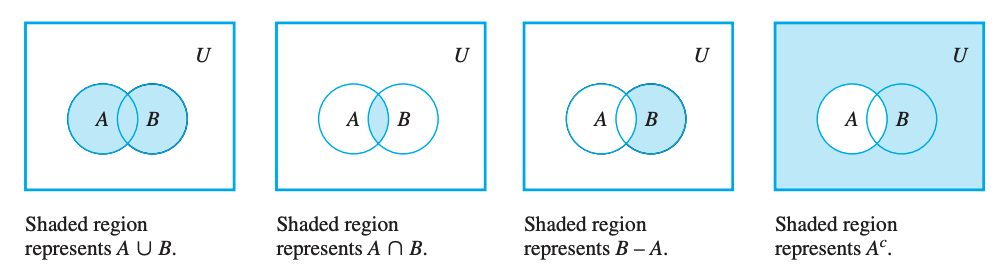
\includegraphics[scale=0.65]{setops}

\subsection{Disjoint Sets and Partitions}

A group of sets are \textbf{mutually disjoint} if the intersection of all pairs of sets is equal to
the empty set $\emptyset$.

\begin{definition}{Partition}{label}
    A finite or infinite collection of nonempty sets $\{A_1, A_2, A_3 \ldots\}$ is a \textbf{partition}
    of a set $A$ if, and only if,
    \begin{enumerate}
        \item $A$ is the union of all the $A_i$
        \item The sets $A_1,A_2,A_3 \ldots$ are mutually disjoint.
    \end{enumerate}
\end{definition}

\begin{definition}{Power Sets}{label}
    Given a set $A$, the \textbf{power set} of $A$, denoted $\wp(A)$, is the set of all subsets of $A$.
\end{definition}

\begin{definition}{Cartesian Product}{label}
    In general, \[
        A_1 \times A_2 \times \ldots A_n = \{(a_1, a_2, \ldots , a_n)  \mid a_1 \in A_1, a_2 \in A_2, \ldots , a_n \in A_n \}
    .\] 
    Note that $A_1 \times A_2 \times A_3$ is not quite the same thing as $(A_1 \times  A_2) \times A_3$
    because of tuple ordering.
\end{definition}

\section{Properties of Sets}

\begin{theorem}{Some Subset Relations}{label}
    \begin{enumerate}
        \item Inclusion of Intersection: $A \cap B \subseteq A$ and vice versa
        \item Inclusion in Union: $A \subseteq A \cup B$ and vice versa
        \item Transitive Property of Subsets: $A \subseteq B \land B \subseteq C \to A \subseteq C$
    \end{enumerate}
    To prove these theorems, \emph{suppose} that there is some arbitrary element of $A$ and show
    that it is also in $B$.
\end{theorem}

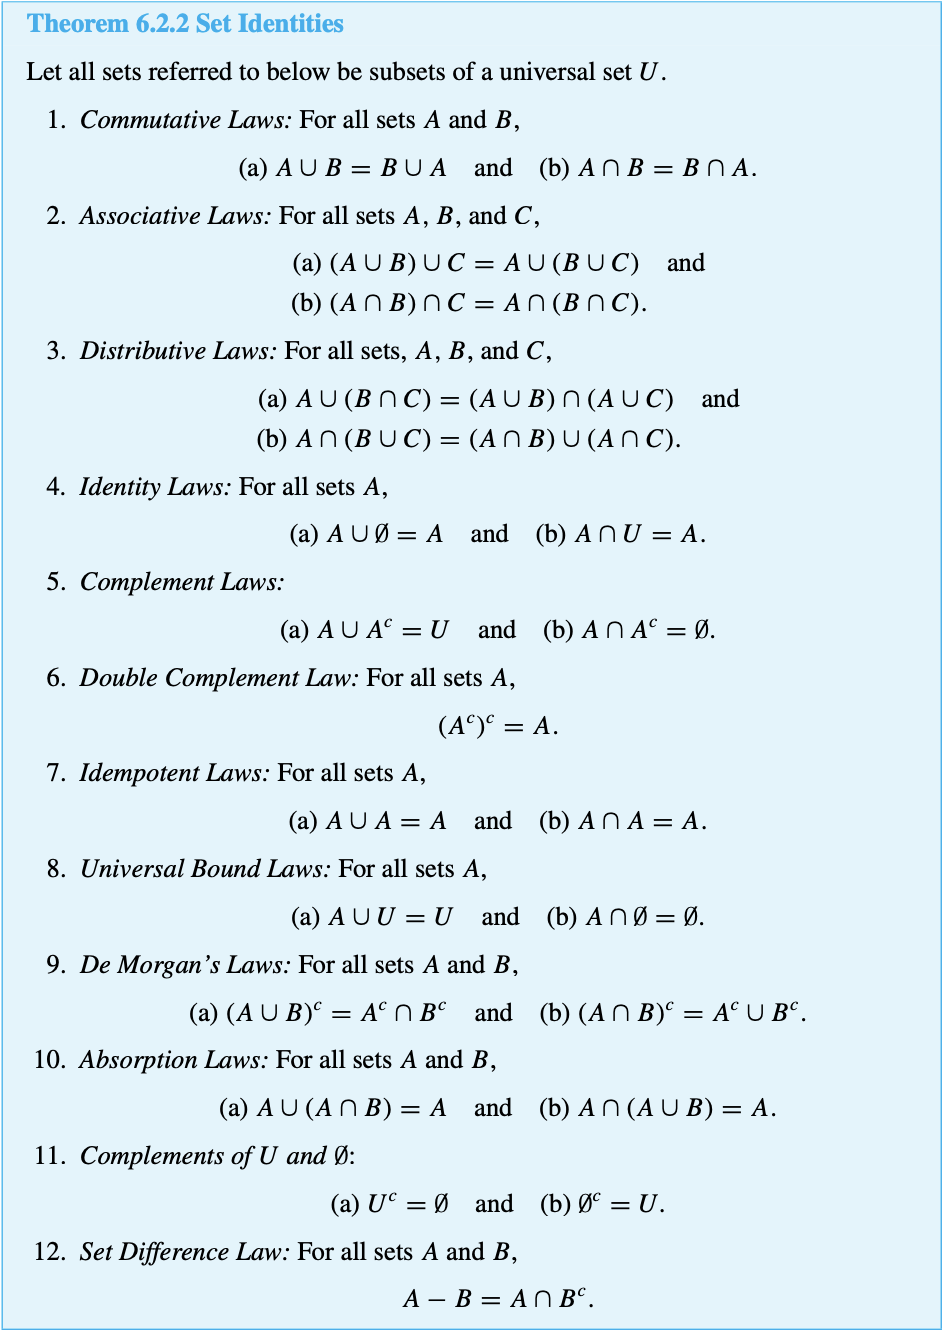
\includegraphics[scale=0.65]{setids}

In general, to prove set equality, you prove that set $A$ is a subset of set $B$, and that
set $B$ is a subset of set $A$. Additionally, to prove that a set $X$ is equal to the empty set
$\emptyset$, suppose $X$ has an element and derive a contradiction.

Additionally, casework is helpful when dealing with unions. It may be helpful to split a union into
2 cases.

\chapter{Functions}

In this chapter we go more in depth into properties of functions and their composition.

\section{Functions Defined on General Sets}

\begin{definition}{Function}{label}
    A \textbf{function} from a set $X$ to a set $Y$, denoted $f: X \to Y$, is a relation from
    $X$, the \textbf{domain}, to $Y$, the \textbf{co-domain}, that satisfies two properties:
    \begin{enumerate}
        \item Every element in $X$ is related to some element in $Y$
        \item No element in $X$ is related to more than one element in $Y$.
    \end{enumerate}
    The set of all values of $f$ is called the \emph{range of f} or the \emph{image of X under f}.
    If there exists some $x$ such that $f(x)=y$, then x is called a \textbf{preimage 
    (or inverse image) of $y$}.

    Two functions $F: X \to Y$ and $G: X \to Y$ are considered equal if, for all $x \in X, F(x) = G(x)$
\end{definition}

\begin{definition}{Identity Function}{label}
    The identity function $I_X$ is a function from $X \to X$ by which $I_X(x) = x \forall x \in X$.
\end{definition}

\begin{definition}{Logarithmic Function}{label}
    The log function $\log_b{x}=y$ (from $\mathbb{R}^{+}$ to $\mathbb{R}$) maps a number to the $y$ in the solution of
    the equation $b^y=x$.
\end{definition}

\subsection{Well Defined Functions}

We say that a function is \textbf{not well defined} if it fails to satisfy at least one of the
requirements for being a function. A function being well defined really means that it qualifies
to be called a function.

\section{One-to-One and Onto, Inverse Functions}

\subsection{One-to-one}

A function is \textbf{one-to-one} (or \textbf{injective}) if, and only if, every input has a unique 
output. Symbolically, $\forall x_1, x_2 \in X, f(x_1)=f(x_2) \to x_1 = x_2$.

To prove that $f$ is one-to-one, you \textbf{suppose} $x_1$ and $x_2$ are elements of $X$ such that
$f(x_1)=f(x_2)$, and \textbf{show} that $x_1=x_2$.

\subsection{Onto}

A function is \textbf{onto} (or \textbf{surjective}) if, and only if, the co-domain of the function
is equal to its image. Symbolically, $\forall y \in Y, \exists x \in X  \mid f(x) = y$.

To prove that $f$ is onto, you \textbf{suppose} $y$ is in $Y$, and \textbf{show} that
there exists an element in $x$ such that $y = f(x)$.

\subsection{One-to-one correspondences and Inverse Functions}

\begin{definition}{Bijection}{label}
    A \textbf{one-to-one correspondence} (or \textbf{bijection}) from a set $X$ to a set $Y$ is
    a function that is both one-to-one and onto.
\end{definition}

\begin{theorem}{Inverse Functions}{label}
    Suppose $F: X \to Y$ is a one-to-one correspondence. Then there is a function $F^{-1}: Y \to X$
    where $F^{-1}(y)=x$. Note that $F^{-1}$ is also a one-to-one correspondence.

    Additionally, note that \[
        f^{-1}(b) = a \Leftrightarrow f(a) = b
    .\] 
\end{theorem}

Finding an inverse function is done while proving that some function $F$ is onto.

\section{Composition of Functions}

The composition of functions (defined as $(g \circ f)(x) = g(f(x)) \forall x \in X$) for two
functions $f: X \to Y$ and $g: Y \to Z$ is $(g \circ f): X \to Z$.
Two compositions are equivalent if they have the same output for every input.

\subsection{Properties of Compositions}

\begin{theorem}{Composition of a Function with Its Inverse}{label}
    $f^{-1} \circ f = I_X$ and $f \circ f^{-1} = I_Y$. This can be proved directly using the
    definition of inverse.
\end{theorem}

\begin{theorem}{One-to-one/Onto Compositions}{label}
    If $f: X \to Y$ and $g: Y \to Z$ are both one-to-one, then $g \circ f$ is one-to-one.
    The same line of reasoning applies for onto functions.
\end{theorem}

\section{Cardinality and Sizes of Infinity}

\begin{definition}{Cardinality}{label}
    Let $A$ and $B$ be any sets. \textbf{$A$ has the same cardinality as $B$} if, and only if, there is
    a one-to-one correspondence from $A$ to $B$. Sets in terms of cardinality follow reflexive,
    symmetric, and transitive properties.
\end{definition}

Note that if a set has the same cardinality as a set that is countably infinite, then the set is
also countably infinite. Surprisingly, the set of all rational numbers is countably infinite.

\subsection{Larger Infinities}

The set of all real numbers is uncountable. This can be proved using the Cantor diagonalization process.
Note that any subset of a countable set is countable, and any subset with an uncountable set is uncountable.

\end{document}
